\section[\thesection \  Evaluierung]{Evaluierung}\label{sec:evaluation}

\begin{frame}{Mean Average Precision (mAP)}
    \fontsize{9pt}{9pt}\selectfont
    \begin{columns}[T]
    \column{0.5\columnwidth}
    \textbf{\normalsize Intersection over Union (IoU)}
    \begin{figure}
        \centering
        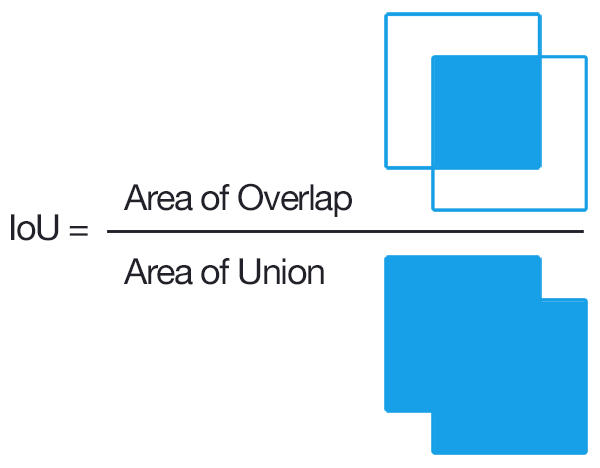
\includegraphics[width=0.7\textwidth]{Bilder/IoU.png}                    
    \end{figure}
    \begin{itemize}
        \item $\text{IoU} > 0.5 \rightarrow \textbf{True Positive}$
    \end{itemize}
    
    \column{0.5\columnwidth}
    \visible<2->{
    \textbf{Recall:} Trefferquote
    \begin{equation*}
        \frac{\text{True Positives}}{\text{alle Objekte im Bild}}
    \end{equation*}
    \\[0.2cm]
    \textbf{Precision} Genauigkeit 
    \begin{equation*}
        \frac{\text{True Positives}}{\text{alle Predictions}}
    \end{equation*}
    \\[0.2cm]
    \textbf{Average Precision} für eine Klasse
    \begin{equation*}
        AP = \frac{1}{N}\sum Precision(Recall)
    \end{equation*}
    }
    \end{columns}
    \visible<3->{
    \normalsize
    \begin{block}{Loss}
        \begin{itemize}
            \item \textbf{Lokalisierung:} Bounding Box Regression
            \item \textbf{Klassifizierung:} (Logarithmische) Fehlerberechnung
        \end{itemize}
        \vspace{0.3cm}
    \end{block}
    }
    
\end{frame}



\begin{frame}{Visualisierung des Trainigsfortschritts}
    \begin{itemize}
        \item Tensorboard
    \end{itemize}
    \begin{columns}[T]
        \column{0.05\textwidth}
        \vspace{1.5cm}
        Loss\\
        \vspace{3cm}
        mAP\\
        

        \column{0.475\textwidth}
        \centering
        \small Ohne Augmentierung
        \begin{figure}
            \centering
            \def\svgwidth{0.7\columnwidth}
            \footnotesize
            \input{Bilder/loss_ohne_aug.pdf_tex}
        \end{figure}

        \begin{figure}
            \centering
            \def\svgwidth{0.7\columnwidth}
            \footnotesize
            \input{Bilder/mAP_ohne_aug.pdf_tex}
        \end{figure}
        

        \column{0.475\textwidth}
        \centering
        \small Mit Augmentierung

        \begin{figure}
            \centering
            \def\svgwidth{0.7\columnwidth}
            \footnotesize
            \input{Bilder/loss_aug.pdf_tex}
        \end{figure}
        \begin{figure}
            \centering
            \def\svgwidth{0.7\columnwidth}
            \footnotesize
            \input{Bilder/mAP_aug.pdf_tex}
        \end{figure}
        
    \end{columns}
\end{frame}



\begin{frame}{Vergleich Modelle: Genauigkeit - Inferenzzeit}
    \begin{columns}
        \column{0.45\columnwidth}
        \textbf{Inferenzzeit auf dem NCS2}


\begin{table}[]
    \begin{tabular}{|lccc|}
    \hline
    \multirow{2}{*}{\begin{tabular}[c]{@{}l@{}}Archi-\\ tecture\end{tabular}} & \multirow{2}{*}{\begin{tabular}[c]{@{}c@{}}Base\\ CNN\end{tabular}} & \multicolumn{2}{c|}{Infer FPS}                          \\
                                                                              &                                                                     & \multicolumn{1}{l}{Sync.} & \multicolumn{1}{l|}{Async.} \\ \hline
    \multirow{2}{*}{SSD}                                                      & Mobilenet                                                           & 12,6                      & 33,6                        \\
                                                                              & InceptionV2                                                         & 10,7                      & \textbf{28,3}               \\ \hline
    \begin{tabular}[c]{@{}l@{}}Faster\\ R-CNN\end{tabular}                    & InceptionV2                                                         & 0,55                      & \textbf{0,72}               \\ \hline
    \end{tabular}
    \end{table}
        
        \column{0.1\columnwidth}
        \column{0.45\columnwidth}

        \visible<2->{
        \textbf{Genauigkeit}
        
        \begin{table}[]
            \begin{tabular}{|lll|}
            \hline
            Model                                                                                             & mAP                                                             & Loss                                                             \\ \hline
            \begin{tabular}[c]{@{}l@{}}SSD InceptionV2\\ +Augmentierung\end{tabular}                          & \begin{tabular}[c]{@{}l@{}}0.55\\ 0.6\end{tabular}              & \begin{tabular}[c]{@{}l@{}}4,4\\ \textbf{4,1}\end{tabular}                \\ \hline
            \begin{tabular}[c]{@{}l@{}}Faster R-CNN\\ +Augmentierung\\ +Dropout/L2 Reg.\end{tabular} & \begin{tabular}[c]{@{}l@{}}0.67\\ 0.7\\ 0.7\end{tabular} & \begin{tabular}[c]{@{}l@{}}0.82\\ 0,7\\ \textbf{0.66}\end{tabular} \\ \hline
            \end{tabular}
            \end{table}
        }
    \end{columns}
    
    \visible<3->{
    \begin{itemize}
        \centering
        \item Je \textbf{genauer}, desto \textbf{langsamer}!
    \end{itemize}
    }
    \end{frame}
